\section{Esempi di test (CLI)}
\begin{enumerate}
  \item Esecuzione del client con server offline \\ \\
  \begin{minipage}[t]{0.3\textwidth}
    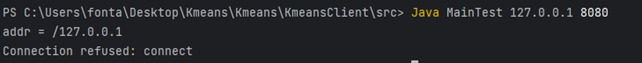
\includegraphics[scale=0.8]{img/test1.png}
  \end{minipage}
  \item Esecuzione senza parametri: il programma deve essere avviato fornendo come parametri l'indirizzo IP/DNS del server e la porta logica. Se si lavora con la stessa macchina si può inserire come primo parametro localhost, 127.0.0.1 (indirizzo IPv4 locale) oppure ::1 (indirizzo IPv6 locale). \\ \\
  \begin{minipage}[t]{0.3\textwidth}
    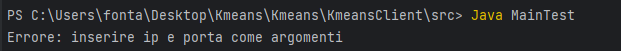
\includegraphics[scale=0.8]{img/test2.png}
  \end{minipage}
  \item Esecuzione con porta errata: la porta logica è un numero a 16 bit, dunque un decimale compreso tra 0 e 65.535. \\ \\
  \begin{minipage}[t]{0.3\textwidth}
    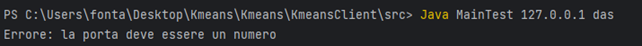
\includegraphics[scale=0.8]{img/test3.png}
  \end{minipage}
  \item Esecuzione con IP/DNS inesistente: in questa esecuzione il server non esiste e dunque il client non riesce a connettersi. In particolare il programma si connette a un server DNS per convertire l'indirizzo fornito in un indirizzo IP ma tale indirizzo non è registrato e dunque si ha errore. \\ \\
  \begin{minipage}[t]{0.3\textwidth}
    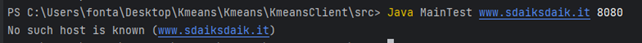
\includegraphics[scale=0.8]{img/test4.png}
  \end{minipage}
  \item Esecuzione con parametri corretti: quando il programma viene eseguito nelle condizioni funzionali (quindi server avviato e parametri validi) vengono stampati a schermo indirizzo IP e porta del server, seguiti dalla porta che sta usando il processo per la comunicazione. Viene poi mostrato all'utente un menù con due opzioni. L'opzione (1) permetterà al client di caricare un cluster di dati che è stato serializzato sul server come un file, mentre l'opzione (2) consente di creare un nuovo cluster di dati mediante l'algoritmo del KMeans. In caso di input non validi viene chiesto all'utente di reinserire finchè non si avrà un'opzione valida.  \\ \\
  \begin{minipage}[t]{0.3\textwidth}
    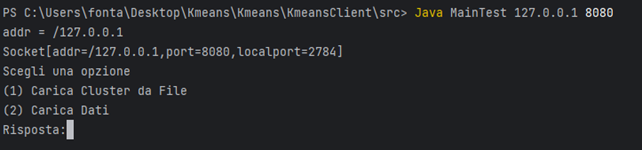
\includegraphics[scale=0.8]{img/test5.png}
  \end{minipage}
  \\
  \begin{minipage}[t]{0.3\textwidth}
    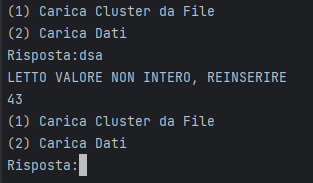
\includegraphics[scale=0.8]{img/test6.png}
  \end{minipage}
  \begin{itemize}[label=-]
    \item \textbf{Opzione (1)}: Viene chiesto all'utente di inserire il nome del database, della tabella e del numero di cluster creati. Il server andrà dunque a cercare il file corrispondente a tali informazioni e, se non trovato, manderà un messaggio di errore all'utente (come nell'esempio). Viene chiesto all'utente se vuole tornare al menù oppure terminare l'esecuzione del programma. Se viene premuto “n” il programma termina. Nel caso in cui il file corrispondente alle richieste esista viene inviato al client il contenuto del file, ovvero i centroidi dei cluster. \\ \\
    \begin{minipage}[t]{0.3\textwidth}
      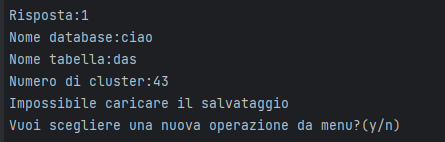
\includegraphics[scale=0.8]{img/test7.png}
    \end{minipage}
    \\
    \begin{minipage}[t]{0.3\textwidth}
      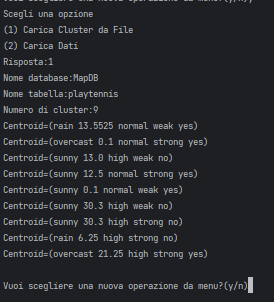
\includegraphics[scale=0.8]{img/test8.png}
    \end{minipage}
    \item \textbf{Opzione (2)}: Viene chiesto all'utente se vuole usare i valori di default o meno per effettuare una prova:
    \begin{itemize}[label=-]
      \item \textbf{Valori di default}: i valori di default sono:
      \begin{itemize}[label=-]
        \item Localhost $\rightarrow$ server database
        \item 3306 $\rightarrow$ porta dabasase
        \item MapDB $\rightarrow$ nome database
        \item Playtennis $\rightarrow$ nome tabella
        \item MapUser $\rightarrow$ nome utente
        \item Map $\rightarrow$ password
      \end{itemize}
      \begin{minipage}[t]{0.3\textwidth}
        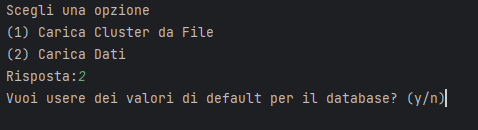
\includegraphics[scale=0.8]{img/test9.png}
      \end{minipage}
      \\ Nel caso di risposta affermativa viene chiesto all'utente il numero dei cluster. Una volta confermati (se questi sono validi) il server eseguirà l'algoritmo di KMeans e invierà il risultato al client. Viene poi chiesto se si vuole riprendere l'esecuzione sullo stesso dataset o meno. \\ \\
      \begin{minipage}[t]{0.3\textwidth}
        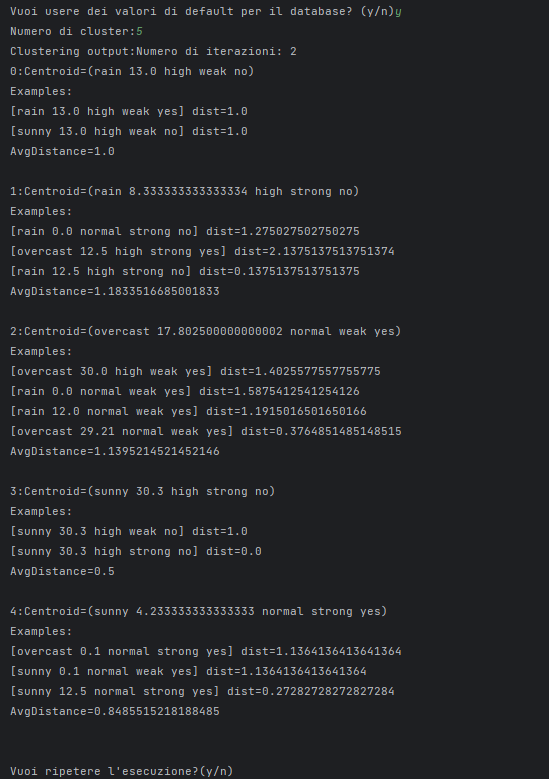
\includegraphics[scale=0.8]{img/test10.png}
      \end{minipage}
      \\ Se l'utente non vuole ripetere l'esecuzione sul dataset ha due scelte:
      \begin{enumerate}
        \item Tornare al menu
        \item Terminare l'esecuzione
      \end{enumerate}
      \begin{minipage}[t]{0.3\textwidth}
        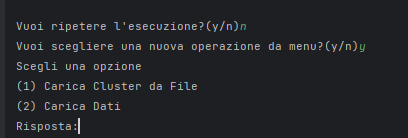
\includegraphics[scale=0.8]{img/test12.png}
      \end{minipage}
      \item \textbf{Valori non di default}: l'utente può scegliere di non usare i valori di default. In quel caso deve inserire tutte le informazioni necessarie. In caso di valori non validi verrà segnalato l'errore all'utente, il quale sceglierà se proseguire con i valori di default oppure se riprovare a inserire dei valori personalizzati. L'uso di valori personalizzati permette di utilizzare dataset già presenti nel server del database. \\ \\
      \begin{minipage}[t]{0.3\textwidth}
        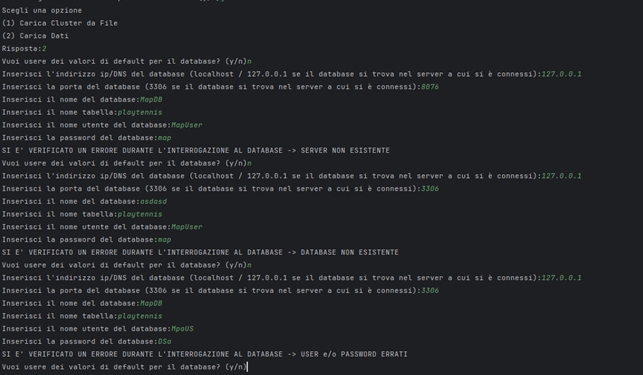
\includegraphics[scale=0.8]{img/test13.png}
      \end{minipage}
    \end{itemize} 
    Ogni volta che l'utente richiede la creazione di un dataset al server, quest'ultimo serializzerà i cluster in un file con nome del tipo: \textbf{\textit{NomeserverNometabellaNumerocluster.dat}}. \\ \\
    \begin{minipage}[t]{0.3\textwidth}
      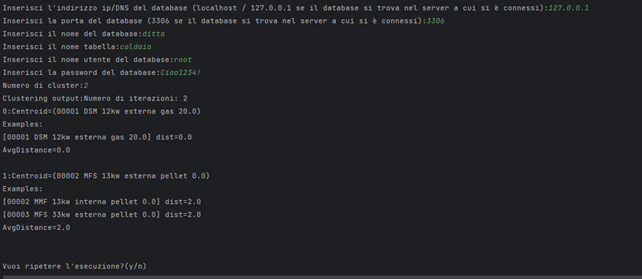
\includegraphics[scale=0.8]{img/test14.png}
    \end{minipage}
  \end{itemize}
\end{enumerate}